\chapter{Software Defined Networking}
\label{sec:chapter_sdn}

Traditional Computer Networks (TCNs) rely on distributed, decentralized architectures where every individual router or switch independently executes both the control plane (e.g., executing Dijkstra's shortest-path calculations via OSPF or IS-IS) and the data plane (hardware-based packet forwarding) \cite{tanenbaum2011computer, bertsekas1992data, kumar2004communication}. While distributed routing protocols offer operational autonomy, they suffer from significant operational inertia: implementing novel traffic engineering policies, modifying forwarding behaviors, or provisioning new Quality-of-Service (QoS) classes requires individual re-configuration of disparate networking devices across the entire autonomous system \cite{vuppalapati2021modeling}.

\textbf{Software Defined Networking (SDN)} fundamentally transforms network management by sundering the control plane from the underlying data plane \cite{vuppalapati2022minimum, vuppalapati2025candidate}. In an SDN architecture, packet forwarding elements (SDN switches) become programmable, simplified hardware execution engines that forward packets strictly according to flow tables populated by a centralized, logically coherent entity known as the \textbf{SDN Controller}. Communication between the controller and the switches is standardized through open interfaces such as the \textbf{OpenFlow} protocol. This centralized global view provides unprecedented agility for dynamic load balancing, real-time traffic redirection, global policy enforcement, and proactive failure recovery.

However, a sudden ``fork-lift'' transition wherein all legacy Internet Protocol (IP) routers are replaced simultaneously by SDN switches is economically prohibitive and operationally hazardous for enterprise and carrier-grade backbones \cite{vuppalapati2022minimum}. Consequently, network operators adopt an incremental deployment strategy, resulting in a coexisting paradigm termed \textbf{Hybrid IP/SDN networks}. In a hybrid IP/SDN architecture, only a strategic subset of routers are replaced by SDN switches (termed \textbf{candidate switches}), while the remainder continue operating legacy hop-by-hop IP routing protocols.

This chapter compiles the comprehensive research contributions on Software Defined Networking conducted by Navya Vuppalapati and T.~G.~Venkatesh \cite{vuppalapati2022minimum, vuppalapati2025candidate, vuppalapati2021modeling, vuppalapati2022gcaiot, vuppalapati2020icacce}. We examine:
\begin{enumerate}
    \item Mathematical formulations and Candidate Selection Algorithms (CSAs) for Single Link Failures (SLFs) under all-shortest-paths modeling;
    \item Resilient candidate selection strategies for simultaneous Multi-Link Failures (MLFs) using Non-Shortest Path (NSP) routing;
    \item Dynamic network scaling algorithms (S-CSA) and budget-constrained deployments (B-CSA);
    \item Queueing-theoretic modeling and transient analysis of SDN controller-switch interactions under non-stationary traffic using Pointwise Stationary Fluid Flow Approximations (PSFFA);
    \item Feedback-based closed-loop congestion control via Proportional-Integral-Derivative (PID) and Dynamic Random Early Detection (DRED) mechanisms.
\end{enumerate}

---

\section{Hybrid IP/SDN Networks and Failure Recovery Architecture}
\label{sec:sdn_hybrid_arch}

Link failures represent frequent and unavoidable occurrences in large-scale computer networks due to physical fiber cuts, hardware degradation, and transient maintenance disruptions \cite{vuppalapati2025candidate}. In legacy IP networks, traditional link recovery relies on \textbf{IP Fast Reroute (IP-FRR)} mechanisms, such as Loop-Free Alternates (LFA) and Not-via addresses. Under IP-FRR, when a router detects an adjacent link failure, it immediately tunnels the impacted traffic to an alternate precomputed node that does not route packets back across the failed link. However, IP-FRR cannot guarantee 100\% failure protection across arbitrary network topologies, often incurs extended repair paths, and severely exacerbates traffic congestion on secondary links.

\begin{figure}[htbp]
    \centering
    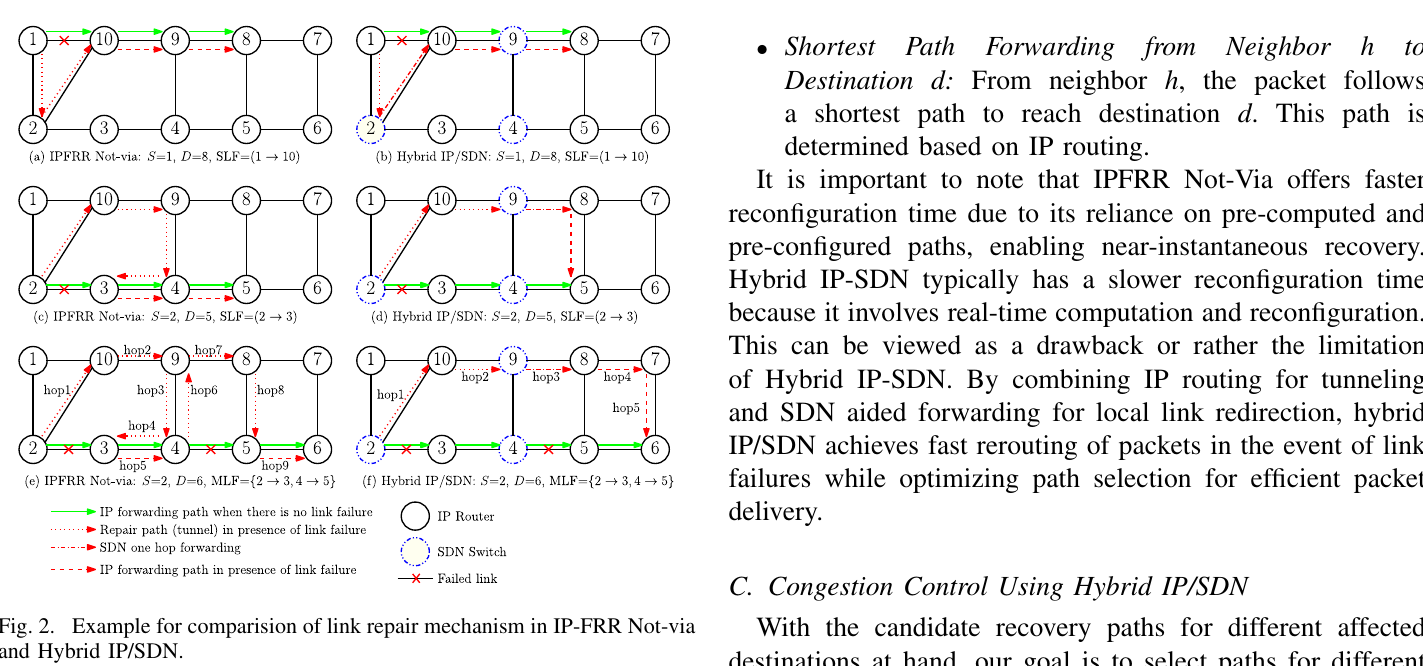
\includegraphics[width=0.85\textwidth]{figures/fig_sdn_repair_mechanism.png}
    \caption{Comparison of link failure recovery mechanisms between traditional IP-FRR (Not-via) and Hybrid IP/SDN architectures \cite{vuppalapati2025candidate}. In hybrid IP/SDN, the detecting node encapsulates packets to a designated SDN candidate switch, which reroutes traffic to destination $D$ avoiding congestion and secondary bottlenecks.}
    \label{fig:sdn_repair_mechanism}
\end{figure}

Hybrid IP/SDN resolves these structural shortcomings through centralized redirection. As illustrated in Figure~\ref{fig:sdn_repair_mechanism}, the recovery process operates through a two-phase protocol:
\begin{enumerate}
    \item \textbf{Encapsulation and Tunneling:} When a directed link $\langle i, j \rangle$ fails, node $i$ (the point of failure detection) encapsulates all affected packets into an IP tunnel addressed to a designated SDN candidate switch $s$. The encapsulation path from $i$ to $s$ traverses the shortest path without crossing the failed link $\langle i, j \rangle$.
    \item \textbf{Decapsulation and Forwarding:} Upon receiving the tunneled packet, the designated SDN candidate switch $s$ strips the encapsulation header, queries its local OpenFlow flow table (populated proactively by the central controller), and forwards the packet along an alternate path to the ultimate affected destination $d$, ensuring the failed link is bypassed entirely.
\end{enumerate}

For this mechanism to function, the network must deploy a sufficient set of candidate SDN switches such that every conceivable link failure is guaranteed to be protected. The critical challenge is the \textbf{Candidate Selection Problem}: determining the minimum number and locations of legacy IP routers to convert into SDN switches to guarantee 100\% link failure protection while optimizing post-recovery performance metrics such as the \textbf{Average Repair Path Length (ARPL)} and the \textbf{Average Maximum Link Utilization (AMLU)} \cite{vuppalapati2022minimum}.

---

\section{Candidate Selection for Single Link Failures (SLFs)}
\label{sec:sdn_slf}

\subsection{System Model and Multi-Shortest Path Formulation}
Consider a network represented by a connected graph $\mathcal{G} = (V, E)$, where $V$ represents the set of nodes ($|V| = N$) and $E$ represents the set of bidirectional links. Each bidirectional link between nodes $i$ and $j$ consists of two unidirectional links denoted by $\langle i, j \rangle$ and $\langle j, i \rangle$. The total number of unidirectional links is $L = 2|E|$.

Prior literature on candidate selection (including the Greedy algorithm of Chu et al., the Search Tree (ST) approach of Li et al., and the Multi-Tunnel (MT) approach of Yang and Yeung) operated under a restrictive assumption: they constructed a single sink tree per destination node, picking only one shortest path at random whenever multiple equal-length shortest paths existed \cite{vuppalapati2022minimum}. Vuppalapati and Venkatesh \cite{vuppalapati2022minimum} demonstrated that this arbitrary tie-breaking artificially inflates the number of affected destinations, leading to suboptimal candidate switch assignments and unnecessarily inflated deployment costs.

To overcome this fundamental limitation, let $\mathcal{T}^{u, v} = \{T_1^{u, v}, T_2^{u, v}, \dots, T_k^{u, v}\}$ denote the complete set of all possible equal-length shortest paths between node $u$ and node $v$. 

\subsection{Affected Destination Set Derivation}
\begin{definition}[\textbf{Affected Destination}]
A node $d \in V$ is defined as an \textbf{affected destination} due to the failure of directed link $\langle i, j \rangle$ if and only if \textit{all} available shortest paths from source $s$ to destination $d$ traverse link $\langle i, j \rangle$, for all $s \in V \setminus \{d\}$.
\end{definition}

The set of all affected destinations associated with the link failure $\langle i, j \rangle$ (or indexed as the $l$-th link failure, $l \in \{1, 2, \dots, L\}$) is denoted by $AD_{\langle i, j \rangle}$ or $AD(l)$:
\begin{equation}
    AD_{\langle i, j \rangle} = \left\{ d \in V \;\middle|\; \forall s \in V \setminus \{d\}, \; \forall T \in \mathcal{T}^{s, d}, \; \langle i, j \rangle \in T \right\}
\end{equation}

By accounting for all equal-cost multipath trajectories, if there exists even a single shortest path between $s$ and $d$ that bypasses $\langle i, j \rangle$, node $d$ is removed from $AD_{\langle i, j \rangle}$. For instance, in the standard Internet2 backbone topology, evaluating the failure of link $\langle 1, 2 \rangle$ under the legacy single-tree approach yields $AD_{\langle 1, 2 \rangle} = \{2, 3, 4, 5, 6\}$ (5 nodes), whereas the exhaustive multipath formulation reveals that alternate equal-length shortest paths exist to nodes 4, 5, and 6 (via $1 \to 10 \to 9$), reducing the true affected destination set strictly to $AD_{\langle 1, 2 \rangle} = \{2, 3\}$. Across the entire Internet2 topology, this lowers the mean number of affected destinations per link failure from $3.46$ down to $2.62$ \cite{vuppalapati2022minimum}.

\subsection{SDN Candidate Table Construction}
A router $k \in V$ is eligible to serve as a designated SDN candidate switch for protecting the directed link failure $\langle i, j \rangle$ if and only if two topological conditions are satisfied simultaneously \cite{vuppalapati2022minimum}:
\begin{enumerate}
    \item \textbf{Ingress Detour Condition:} Among all available shortest paths from the failure-detecting node $i$ to candidate switch $k$, there exists at least one shortest path that does not contain the failed link $\langle i, j \rangle$.
    \item \textbf{Egress Forwarding Condition:} For every affected destination $d \in AD_{\langle i, j \rangle}$, there exists at least one neighbor node $h \in \mathcal{N}(k)$ adjacent to $k$ such that an available shortest path from $h$ to $d$ does not contain the failed link $\langle i, j \rangle$.
\end{enumerate}

Based on these dual criteria, an $L \times N$ binary \textbf{SDN Candidate Table} $\mathbf{T}$ is formed:
\begin{equation}
    T(l, n) = \begin{cases}
        1, & \text{if node } n \text{ satisfies Conditions 1 and 2 for the } l\text{-th link failure}, \\
        0, & \text{otherwise}.
    \end{cases}
\end{equation}

\subsection{The Minimum Candidate Selection (MCS) Algorithm}
Let $\mathcal{C}$ denote the family of candidate sets. A subset of nodes $C \subseteq V$ forms a valid candidate set if and only if every link failure $l \in \{1, 2, \dots, L\}$ is covered by at least one node in $C$:
\begin{equation}
    \bigvee_{n \in C} T(l, n) = 1, \quad \forall l \in \{1, 2, \dots, L\}
\end{equation}

The \textbf{Minimum Candidate Selection (MCS)} algorithm, formulated in Algorithm~\ref{alg:mcs}, determines candidate sets of absolute minimal cardinality through an incremental combinatorial evaluation.

\begin{algorithm}[htbp]
\caption{Minimum Candidate Selection (MCS) Algorithm \cite{vuppalapati2022minimum}}
\label{alg:mcs}
\begin{algorithmic}[1]
\Require Binary candidate table $\mathbf{T} \in \{0, 1\}^{L \times N}$
\Ensure Family of minimal SDN candidate sets $\mathcal{C}$
\State Initialize $\mathcal{C} \gets \emptyset$
\For{$i = 1$ to $N$}
    \State Form combination matrix $\mathbf{M}_i$ of size $\binom{N}{i} \times i$, where each row is an $i$-combination of $\{1, 2, \dots, N\}$
    \For{$j = 1$ to $\binom{N}{i}$}
        \State $\mathbf{OR\_arr} \gets [0, 0, \dots, 0]^T$ of length $L$
        \For{$k = 1$ to $i$}
            \State $\mathbf{OR\_arr} \gets \mathbf{OR\_arr} \;\lor\; \mathbf{T}_{:, M_i(j, k)}$ \Comment{Bitwise logical OR of columns}
        \EndFor
        \If{$\sum_{l=1}^L OR\_arr(l) = L$}
            \State $\mathcal{C} \gets \mathcal{C} \cup \{\text{row } j \text{ of } \mathbf{M}_i\}$
        \EndIf
    \EndFor
    \If{$\mathcal{C} \neq \emptyset$}
        \State \textbf{break} \Comment{Minimal cardinality found; terminate search}
    \EndIf
\EndFor
\State \Return $\mathcal{C}$
\end{algorithmic}
\end{algorithm}

\subsection{Candidate Set Selection: MCS-ARPL and MCS-AMLU}
Because Algorithm~\ref{alg:mcs} can produce multiple candidate sets $\mathcal{C} = \{C_1, C_2, \dots\}$ sharing the same minimal cardinality, a secondary selection objective must be applied. Vuppalapati and Venkatesh formulated two targeted optimization schemes:

\subsubsection{1. Average Repair Path Length Minimization (MCS-ARPL)}
For a candidate set $C_m \in \mathcal{C}$ and link failure $l$, let $rps_{s, d}^{(l)}$ denote the repair path length from node $i$ to destination $d \in AD(l)$ when candidate switch $s \in C_m$ is utilized. The average repair path length for link failure $l$ under candidate $s$ is:
\begin{equation}
    RP_s^{(l)} = \begin{cases}
        \frac{1}{|AD(l)|} \sum_{d \in AD(l)} rps_{s, d}^{(l)}, & \text{if } T(l, s) = 1, \\
        0, & \text{if } T(l, s) = 0.
    \end{cases}
\end{equation}

The optimal candidate switch $s_m^{(l)} \in C_m$ mapped to link failure $l$ is chosen to minimize this path length:
\begin{equation}
    s_m^{(l)} = \arg\min_{s \in C_m, T(l, s) = 1} RP_s^{(l)}
\end{equation}

The network-wide Average Repair Path Length for candidate set $C_m$ is then:
\begin{equation}
    RP_m = \frac{1}{L} \sum_{l=1}^L RP_{s_m^{(l)}}^{(l)}
\end{equation}

The final optimal candidate set $C^*$ under MCS-ARPL is:
\begin{equation}
    C^*_{\text{ARPL}} = \arg\min_{C_m \in \mathcal{C}} RP_m
\end{equation}

\subsubsection{2. Load Balancing via Maximum Link Utilization (MCS-AMLU)}
To prevent traffic bottlenecks during failover, the **MCS-AMLU** algorithm maps link failures to candidates that minimize the post-recovery \textbf{Average Maximum Link Utilization (AMLU)}. Let $U_{\max}(l, s)$ denote the highest link utilization observed across all operational links in $\mathcal{G}$ when link $l$ fails and traffic is rerouted through candidate $s$. The optimal candidate set $C^*_{\text{AMLU}}$ is selected via:
\begin{equation}
    C^*_{\text{AMLU}} = \arg\min_{C_m \in \mathcal{C}} \left( \frac{1}{L} \sum_{l=1}^L \min_{s \in C_m, T(l, s)=1} U_{\max}(l, s) \right)
\end{equation}

---

\section{Candidate Selection under Multi-Link Failures (MLFs)}
\label{sec:sdn_mlf}

While single link failures account for the majority of isolated disruptions, real-world backbones frequently suffer concurrent \textbf{Multi-Link Failures (MLFs)} caused by shared risk link groups (SRLGs), correlated power outages, or severe environmental disasters \cite{vuppalapati2025candidate}. Let an MLF event involving $K$ simultaneous link failures be denoted by:
\begin{equation}
    F_m = \{slf_1, slf_2, \dots, slf_K\} \subset E, \quad |F_m| = K
\end{equation}

\subsection{The Zero-Row Vulnerability and Non-Shortest Path (NSP) Approach}
When evaluating MLF scenarios under conventional shortest-path routing, a critical breakdown occurs: for many simultaneous failure combinations, every shortest path to candidate switches or affected destinations traverses at least one of the failed links in $F_m$. Consequently, the corresponding row in the candidate table contains all zeros ($\mathbf{T}_{m, :} = \mathbf{0}$), making complete failure protection impossible \cite{vuppalapati2025candidate}. In the Internet2 topology with $K = 2$, exactly 20 MLF combinations produce all-zero candidate rows under shortest-path routing.

To overcome this fundamental obstacle, Vuppalapati and Venkatesh \cite{vuppalapati2025candidate} conceived the \textbf{Non-Shortest Path (NSP)} framework. Rather than restricting detour routes strictly to equal-length shortest paths, the NSP algorithm considers paths with incrementally longer hop counts. 

Let all simple paths from source $s$ to destination $d$ be ordered according to their unique path lengths:
\begin{equation}
    \text{path\_len\_unique} = \{\ell_1, \ell_2, \dots, \ell_U\}, \quad \text{where } \ell_1 < \ell_2 < \dots < \ell_U
\end{equation}
Each length level is indexed by the \textbf{Shortest Path Index} ($sp\_idx \in \{1, 2, \dots\}$), where $sp\_idx = 1$ denotes standard shortest paths, $sp\_idx = 2$ includes the next-shortest simple paths, and so forth.

Under an MLF $F_m$ and given $sp\_idx$, destination $d$ belongs to the affected destination set $AF_m$ if and only if \textit{every} simple path with index up to $sp\_idx$ traverses at least one failed link in $F_m$:
\begin{equation}
    AF_m(sp\_idx) = \left\{ d \in V \;\middle|\; \forall P \in \mathcal{P}_{sp\_idx}^{s, d}, \; P \cap F_m \neq \emptyset, \; \forall s \in V \setminus \{d\} \right\}
\end{equation}
Incrementing $sp\_idx$ allows detour traffic to route through non-shortest simple paths, successfully populating previously empty rows in the candidate table and restoring 100\% MLF protection.

\subsection{Four Unified MLF Candidate Selection Algorithms}
To derive candidate sets from the NSP candidate table, Vuppalapati and Venkatesh proposed four distinct algorithmic strategies balancing computational complexity and optimality:
\begin{enumerate}
    \item \textbf{G-FTU (Greedy with Full Table Update):} Formulates the complete candidate table across all MLFs using the NSP approach, and executes a greedy column-sum selection. After each candidate node is picked, all covered MLF rows are eliminated, and column sums are recomputed iteratively until all MLFs are protected.
    \item \textbf{M-FTU (Minimum Candidate Selection with Full Table Update):} Employs the exhaustive combinatorial search of Algorithm~\ref{alg:mcs} on the fully populated NSP candidate table, guaranteeing the mathematically minimal candidate set size.
    \item \textbf{G-PTU (Greedy with Partial Table Update):} Avoids the heavy computational overhead of constructing the entire NSP table beforehand. It initializes with standard shortest paths ($sp\_idx = 1$), detects zero-rows on demand, and updates only the necessary partial rows using higher $sp\_idx$ levels before executing greedy selection.
    \item \textbf{M-PTU (Minimum Candidate Selection with Partial Table Update):} Executes the exact MCS combinatorial search over a partially expanded candidate table, providing minimal candidate sizes with dramatically reduced preprocessing runtimes.
\end{enumerate}

\subsection{Dynamic Network Scaling (S-CSA)}
When networks expand—such as when new autonomous nodes or high-bandwidth links are added to an existing backbone—recomputing the entire candidate set from scratch is impractical and financially disruptive. The **Scaling Candidate Selection Algorithm (S-CSA)** preserves all previously deployed SDN candidate switches $C_{\text{old}}$ and determines only the minimal additional candidate switches $\Delta C$ required to cover the new links $\Delta E$.

\begin{figure}[htbp]
    \centering
    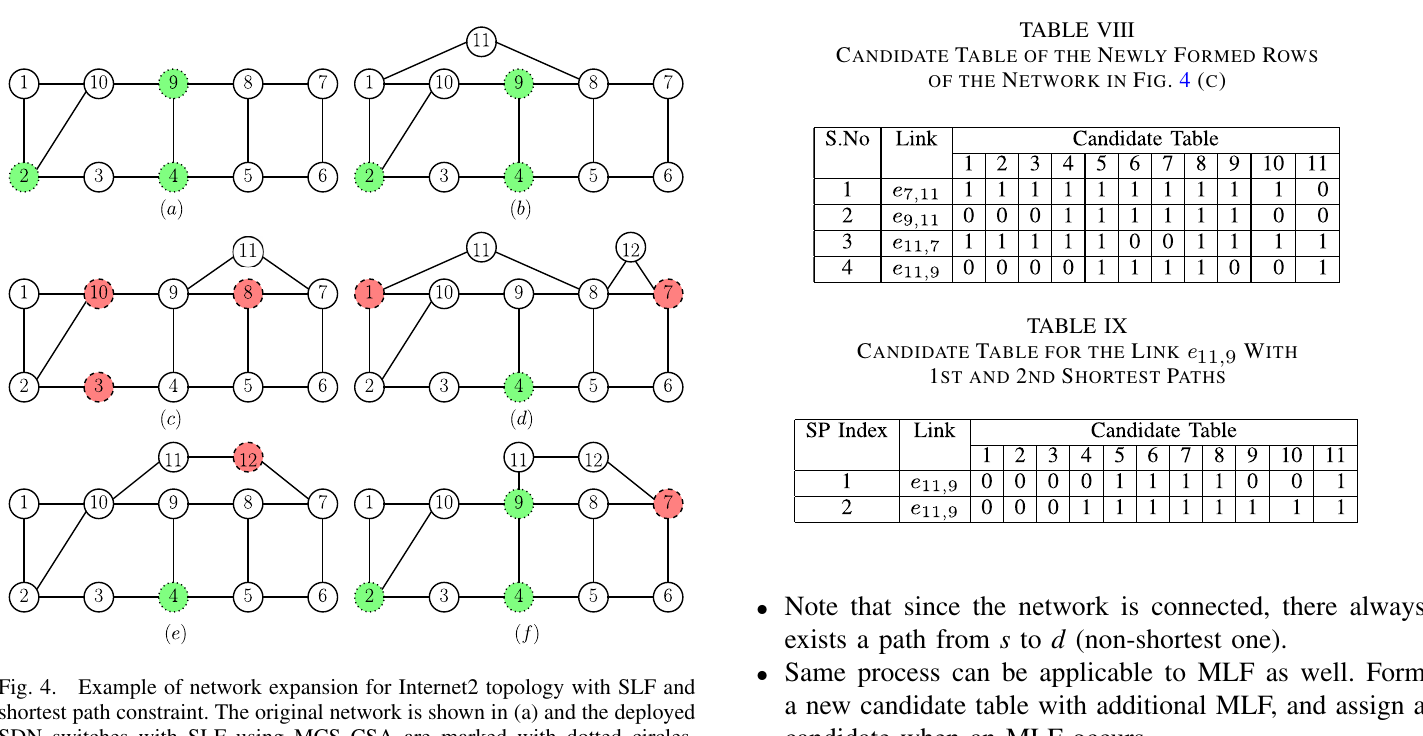
\includegraphics[width=0.85\textwidth]{figures/fig_sdn_network_expansion.png}
    \caption{Example of network scaling and expansion on the Internet2 topology \cite{vuppalapati2025candidate}. Baseline deployed SDN switches are maintained while new nodes (11 and 12) and associated links are incrementally protected with minimal additional candidate switches.}
    \label{fig:sdn_network_expansion}
\end{figure}

As shown in Figure~\ref{fig:sdn_network_expansion}, when new nodes 11 and 12 are integrated into the Internet2 topology, S-CSA verifies whether the existing candidate set $\{2, 4, 9\}$ can protect the newly formed links. If new failure scenarios remain unprotected, S-CSA selects additional candidates from the newly added nodes, ensuring seamless scaling without re-engineering existing control infrastructure.

\subsection{Budget-Constrained Candidate Selection (B-CSA)}
In operational environments governed by strict capital expenditure (CAPEX) limits, the available budget $B$ may be lower than the minimal cardinality $|C^*|$ required for 100\% failure protection. To address this scenario, Vuppalapati, Venkatesh, and Gupta \cite{vuppalapati2022gcaiot, vuppalapati2025candidate} formulated the \textbf{Budget-Constrained Candidate Selection Algorithm (B-CSA)}.

Given a budget allowing at most $B$ candidate switches ($B < |C^*|$), B-CSA optimizes failure coverage $\Gamma(C)$ while minimizing the post-recovery repair path length:
\begin{align}
    \max_{C \subset V, |C| \le B} \quad & \Gamma(C) = \frac{1}{|F|} \sum_{m=1}^{|F|} \left( \bigvee_{n \in C} T(m, n) \right) \\
    \text{subject to} \quad & \text{ARPL}(C) \le \text{ARPL}_{\text{threshold}}
\end{align}
Conversely, when budget surplus exists ($B > |C^*|$), B-CSA allocates redundant candidate switches to maximize traffic distribution and minimize link utilization variance across the network \cite{vuppalapati2022gcaiot}.

---

\section{Traffic Characterization and Non-Stationary Fluid Flow Modeling}
\label{sec:sdn_nonstationary}

\subsection{Augmented Dickey-Fuller (ADF) Traffic Characterization}
A core assumption in classical queueing models of communication networks is that packet arrival processes are stationary, meaning their statistical moments (mean, variance, autocorrelation) remain invariant over time \cite{gross2018fundamentals, kleinrock1975queueing1}. However, in SDN architectures, frequent flow rule updates, controller queries, dynamic service provisioning, and reactive rerouting induce severe non-stationarity into control-plane and data-plane traffic \cite{vuppalapati2021modeling, vuppalapati2020icacce}.

Vuppalapati and Venkatesh \cite{vuppalapati2021modeling} conducted formal statistical validation of SDN traffic using the **Augmented Dickey-Fuller (ADF) test**. The ADF test evaluates whether a time-series traffic trace $Y_t$ possesses a unit root (indicating non-stationarity):
\begin{equation}
    \Delta Y_t = \alpha + \beta t + \gamma Y_{t-1} + \sum_{i=1}^p \delta_i \Delta Y_{t-i} + \varepsilon_t
\end{equation}
where the null hypothesis $H_0: \gamma = 0$ corresponds to a non-stationary unit-root process, and the alternative hypothesis $H_1: \gamma < 0$ corresponds to stationary behavior. Empirical testing on real-world SDN traces under dynamic service shifts revealed ADF test statistics failing to reject $H_0$ ($p > 0.05$), confirming that SDN traffic inherently exhibits non-stationary dynamics that defeat conventional steady-state queueing formulations \cite{vuppalapati2021modeling}.

\subsection{Pointwise Stationary Fluid Flow Approximation (PSFFA)}
To capture the time-dependent evolution of queue backlogs at both SDN switches and the central controller, Vuppalapati and Venkatesh \cite{vuppalapati2021modeling} developed a transient queueing model using the **Pointwise Stationary Fluid Flow Approximation (PSFFA)**.

\begin{figure}[htbp]
    \centering
    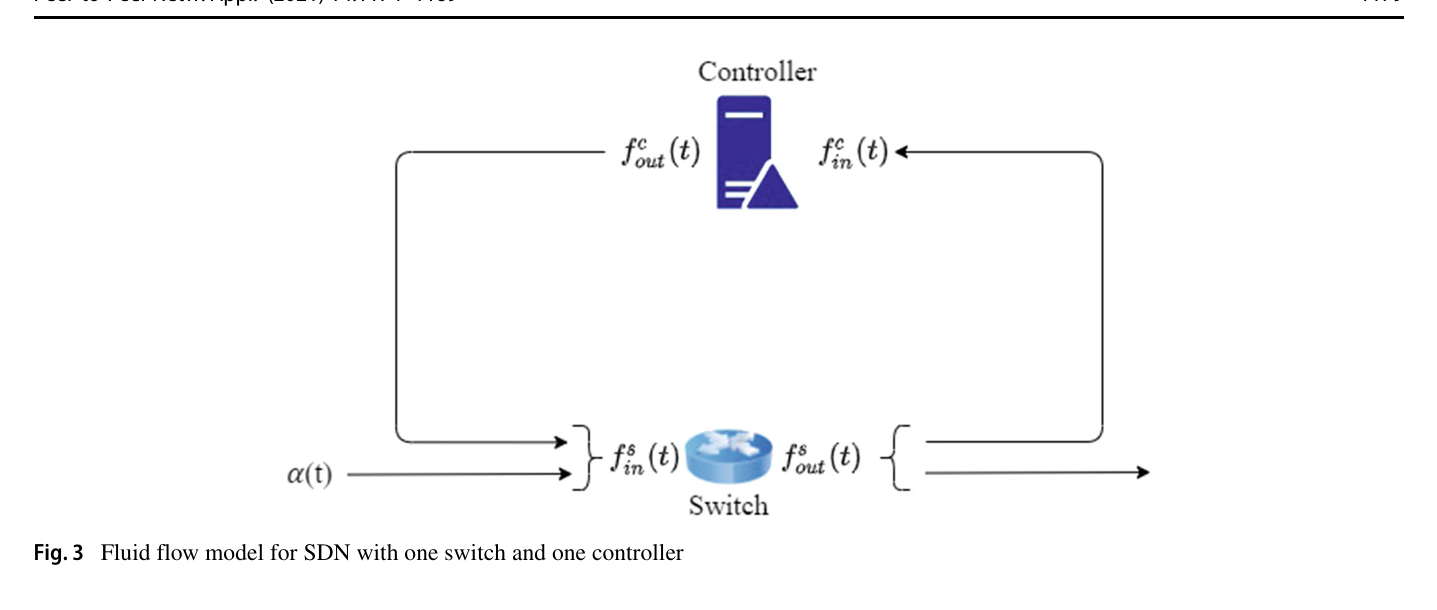
\includegraphics[width=0.85\textwidth]{figures/fig_sdn_fluid_flow_model.png}
    \caption{Fluid flow queueing model for an SDN architecture comprising an OpenFlow switch and a centralized controller under time-varying, non-stationary traffic \cite{vuppalapati2021modeling}.}
    \label{fig:sdn_fluid_flow_model}
\end{figure}

As illustrated in Figure~\ref{fig:sdn_fluid_flow_model}, consider an OpenFlow switch coupled with a central controller:
\begin{itemize}
    \item External time-varying traffic enters the switch at rate $\alpha(t)$ (packets/s).
    \item When a packet arrives without an active flow rule (a table-miss), a \textit{Packet-In} message is dispatched to the controller. Let $q$ denote the fraction of external arrivals directed to the controller ($0 \le q \le 1$).
    \item The service rates of the switch and controller are denoted by $\mu_s$ and $\mu_c$, respectively.
    \item The state variables $x_s(t)$ and $x_c(t)$ represent the ensemble average queue length (number of packets) at time $t$ in the switch and controller, respectively.
\end{itemize}

Applying the flow conservation principle, the instantaneous rate of change of fluid backlogs is governed by coupled ordinary differential equations:
\begin{align}
    \frac{dx_s(t)}{dt} &= -f_{\text{out}}^s(t) + f_{\text{in}}^s(t) \\
    \frac{dx_c(t)}{dt} &= -f_{\text{out}}^c(t) + f_{\text{in}}^c(t)
\end{align}

Accounting for external arrivals, controller flow modifications, and time-dependent link utilization factors $\rho_s(t)$ and $\rho_c(t)$:
\begin{align}
    f_{\text{in}}^s(t) &= \alpha(t) + f_{\text{out}}^c(t) = \alpha(t) + \mu_c \rho_c(t) \\
    f_{\text{in}}^c(t) &= q \, \alpha(t) \\
    f_{\text{out}}^s(t) &= \mu_s \rho_s(t)
\end{align}

Under PSFFA, the instantaneous utilization is expressed as a continuous mapping $G(x(t))$ derived from the steady-state equilibrium of the underlying queueing discipline \cite{vuppalapati2021modeling}. For a Markovian service system ($M_t/M/1$), the equilibrium queue backlog satisfies $x = \rho / (1 - \rho)$, yielding the utilization function:
\begin{equation}
    G(x(t)) = \frac{x(t)}{x(t) + 1}
\end{equation}

Substituting into the conservation equations yields the coupled non-linear differential system:
\begin{align}
    \frac{dx_s(t)}{dt} &= -\mu_s \left( \frac{x_s(t)}{x_s(t) + 1} \right) + \alpha(t) + \mu_c \left( \frac{x_c(t)}{x_c(t) + 1} \right) \label{eq:psffa_switch} \\
    \frac{dx_c(t)}{dt} &= -\mu_c \left( \frac{x_c(t)}{x_c(t) + 1} \right) + q \, \alpha(t) \label{eq:psffa_controller}
\end{align}

Equations~(\ref{eq:psffa_switch}) and (\ref{eq:psffa_controller}) describe the complete transient trajectories of both switch and controller queues under arbitrary non-stationary arrival profiles $\alpha(t)$ (such as step surges, sinusoidal daily variations, or bursty Pareto shocks) without requiring computationally expensive discrete-event simulations \cite{vuppalapati2021modeling}.

\subsection{Closed-Loop Congestion Control: PID and DRED Mechanisms}
Under sudden traffic surges, controller queue backlogs explode, causing delayed flow table installations and severe buffer drops at switches. To maintain queue stability under non-stationary traffic, Vuppalapati and Venkatesh \cite{vuppalapati2021modeling} synthesized two active closed-loop control algorithms:

\subsubsection{1. Proportional-Integral-Derivative (PID) Controller}
The controller monitors its instantaneous queue length $x_c(t)$ against a target reference setpoint $x_{\text{ref}}$. The tracking error is:
\begin{equation}
    e(t) = x_{\text{ref}} - x_c(t)
\end{equation}

The control output $u(t)$ dynamically modulates the controller's admission or packet-in processing probability:
\begin{equation}
    u(t) = K_p \, e(t) + K_i \int_0^t e(\tau) \, d\tau + K_d \, \frac{de(t)}{dt}
\end{equation}
where $K_p$, $K_i$, and $K_d$ represent proportional, integral, and derivative gains tuned to ensure asymptotic stability and eliminate steady-state offsets under non-stationary driving inputs.

\subsubsection{2. Dynamic Random Early Detection (DRED)}
As an alternative, a DRED-based queue thresholding mechanism calculates the error difference between $x_c(t)$ and the setpoint $x_{\text{ref}}$ over discrete sampling epochs, adaptively updating the random packet-in drop probability $p_d(k)$ to preemptively throttle switch traffic before buffer overflow occurs \cite{vuppalapati2021modeling}.

---

\section{Empirical Evaluation and Topology Benchmarks}
\label{sec:sdn_results}

The performance of the proposed candidate selection and transient SDN modeling algorithms has been validated extensively across multiple canonical carrier backbone topologies \cite{vuppalapati2022minimum, vuppalapati2025candidate}, summarized in Table~\ref{tab:sdn_topologies}.

\begin{table}[htbp]
\centering
\caption{Characteristics of standard backbone network topologies evaluated in Hybrid IP/SDN studies \cite{vuppalapati2022minimum, vuppalapati2025candidate}.}
\label{tab:sdn_topologies}
\begin{tabular}{lcccc}
\toprule
\textbf{Network Topology} & \textbf{Nodes ($N$)} & \textbf{Bidirectional Links ($|E|$)} & \textbf{Unidirectional Links ($L$)} \\
\midrule
Internet2   & 10 & 14 & 28 \\
Abilene     & 12 & 15 & 30 \\
NSFNet      & 14 & 21 & 42 \\
AttMpls     & 25 & 56 & 112 \\
\bottomrule
\end{tabular}
\end{table}

The primary findings from extensive simulations and numerical analyses are summarized below:
\begin{itemize}
    \item \textbf{Candidate Switch Minimization:} The MCS algorithm consistently identifies candidate sets that are strictly smaller than or equal to those computed by legacy Greedy, Search Tree (ST), and Multi-Tunnel (MT) algorithms across all topologies \cite{vuppalapati2022minimum}.
    \item \textbf{Significant Repair Path Reduction:} Under Multi-Link Failures ($K \ge 2$), the Non-Shortest Path (NSP) based candidate selection algorithms achieve substantial reductions in Average Repair Path Length (ARPL) compared to baseline IP-FRR and shortest-path approaches: reducing ARPL by \textbf{31.37\%} in NSFNet, \textbf{22.15\%} in AttMpls, and \textbf{18.64\%} in Abilene \cite{vuppalapati2025candidate}.
    \item \textbf{Load Balancing and Congestion Avoidance:} By optimizing the MCS-AMLU metric, maximum post-recovery link utilizations remain well below link capacity thresholds, preventing secondary cascade dropouts.
    \item \textbf{Transient Stability:} PSFFA fluid approximations match discrete-event simulation backlogs with over 98\% accuracy while reducing computational runtime by orders of magnitude. The PID feedback mechanism reliably clamps controller queue fluctuations within 5\% of the target setpoint even under 300\% transient arrival surges \cite{vuppalapati2021modeling}.
\end{itemize}

---

\section{Summary}
\label{sec:sdn_summary}

Software Defined Networking introduces centralized programmability and agile control to modern communication backbones. However, practical deployment requires careful architectural transition through hybrid IP/SDN networks and rigorous transient queue management.

The contributions detailed in this chapter provide an end-to-end analytical and algorithmic framework for SDN:
\begin{enumerate}
    \item The **Minimum Candidate Selection (MCS)** algorithm leverages all-shortest-paths modeling to minimize the number of legacy IP routers requiring upgrade to SDN switches under single link failures.
    \item The **Non-Shortest Path (NSP)** framework resolves the zero-row failure bottleneck under concurrent multi-link disruptions, enabling robust failure protection across four complementary table update algorithms (G-FTU, M-FTU, G-PTU, M-PTU).
    \item The **S-CSA** and **B-CSA** algorithms extend practical applicability to dynamic network expansion and strict financial CAPEX budgets.
    \item The **PSFFA fluid flow model** provides accurate transient analysis of controller-switch queue dynamics under non-stationary traffic, while PID feedback control ensures robust stability against traffic spikes.
\end{enumerate}
These techniques establish a rigorous mathematical foundation for the scalable, resilient, and economically viable deployment of next-generation software-defined carrier networks.
